\chapter{METODOLOGIA}\label{chp:METODOLOGIA}

Nesta seção, descreve-se como o trabalho foi desenvolvido, explicitando sucintamente a metodologia, os materiais e processos empregados para a execução do trabalho e como os objetivos serão alcançados. Esta seção responde às perguntas: Como será feita a pesquisa? Com o quê? Como será procedida a pesquisa? Visa a explicar de forma detalhada todas as ações desenvolvidas no percurso da pesquisa para que possa ser validada como científica. Então, esta seção descreve um método ou adapta uma metodologia preexistente. 

Para os trabalhos que envolvem pesquisas de campo, devem ser apresentados os instrumentos utilizados (questionário abertos, semiabertos, estruturados etc.) e a pertinência deles para o objeto de investigação proposto no trabalho, para que a pesquisa seja atestada como científica. Nesse caso, deve-se responder: Quais são os caminhos para se chegar aos objetivos propostos? Qual é o tipo de pesquisa? Qual é o universo da pesquisa? Será utilizada a amostragem? Quais são os instrumentos de coleta de dados?  Como foram construídos os instrumentos de pesquisa? Que forma é usada para a tabulação de dados? Como serão interpretados e analisados os dados e informações? 

 \section{ESTRUTURA DE UM TRABALHO ACADÊMICO}\label{sec:ESTRUTURATRAB}
A organização de um trabalho acadêmico obedece a normas adotadas pela instituição (Figura \ref{fig:EstruturaTrab}). Tais normas garantem a organização do trabalho e guiam o autor.

\begin{figure}[htb]
	\centering
	\caption{Estrutura para elaboração de trabalhos acadêmicos.}
	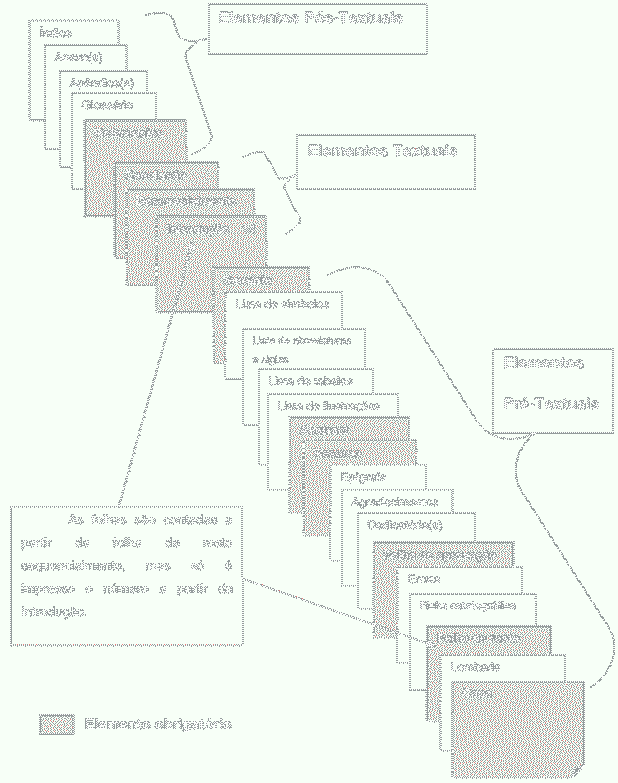
\includegraphics[scale=0.6]{imagens/Estrutura-Trabalhos.png} 
	\newline \textbf{Fonte}: \cite{webLink}.
	\label{fig:EstruturaTrab}
\end{figure}

\section{TEMÁTICA DO TCC}\label{sec:TEMÁTICATCC}
Os temas tratados no TCC devem estar relacionados ao objeto de estudo da Ciência da Computação e estar inseridos em suas subáreas (Quadro 2) e abordar um problema do mundo real, a fim de propor soluções e melhorias. O TCC deve relacionar conhecimentos adquiridos em várias das disciplinas cursadas. Por exemplo, podem envolver algumas das seguintes áreas: inteligência artificial, redes, robótica, pesquisa operacional, grafos, arquitetura de \textit{hardware}, paradigmas de linguagens de programação, comunicação de dados, computação gráfica, matemática/estatística.  

\begin{table}[t]
	\caption{Áreas que compõem a Ciência da Computação de acordo com o CNPQ.}
	\label{tab:AreasCNPQ}
	\begin{tabular}{|l|l|}
		\hline
		\textbf{10300007} & \textbf{CIÊNCIA DA COMPUTAÇÃO}                     \\ \hline
		10301003          & TEORIA DA COMPUTAÇÃO                               \\ \hline
		10301011          & COMPUTABILIDADE E MODELOS DE COMPUTAÇÃO            \\ \hline
		10301020          & LINGUAGEM FORMAIS E AUTÔMATOS                      \\ \hline
		10301038          & ANÁLISE DE ALGORITMOS E COMPLEXIDADE DE COMPUTAÇÃO \\ \hline
		10301046          & LÓGICAS E SEMÂNTICA DE PROGRAMAS                   \\ \hline
		10302000          & MATEMÁTICA DA COMPUTAÇÃO                           \\ \hline
		10302018          & MATEMÁTICA SIMBÓLICA                               \\ \hline
		10302026          & MODELOS ANALÍTICOS E DE SIMULAÇÃO                  \\ \hline
		10303006          & METODOLOGIA E TÉCNICAS DA COMPUTAÇÃO               \\ \hline
		10303014          & LINGUAGENS DE PROGRAMAÇÃO                          \\ \hline
		10303022          & ENGENHARIA DE SOFTWARE                             \\ \hline
		10303030          & BANCO DE DADOS                                     \\ \hline
		10303049          & SISTEMAS DE INFORMAÇÃO                             \\ \hline
		10303057          & PROCESSAMENTO GRÁFICO (GRAPHICS)                   \\ \hline
		10304002          & SISTEMA DE COMPUTAÇÃO                              \\ \hline
		10304010          & HARDWARE                                           \\ \hline
		10304029          & ARQUITETURA DE SISTEMAS DE COMPUTAÇÃO              \\ \hline
		10304037          & SOFTWARE BÁSICO                                    \\ \hline
		10304045          & TELEINFORMÁTICA                                    \\ \hline
	\end{tabular}
	\newline \footnotesize \textbf{Fonte: \cite{Capes2018}.}
\end{table}

\section{SUGESTÕES DE FORMATOS DE TCC}\label{sec:SUGESTOESTCC}
Os TCCs do curso de Bacharelado em Ciência da Computação podem tratar de desenvolvimento de \textit{softwares} comerciais; desenvolvimento de \textit{softwares} científicos; desenvolvimento de \textit{softwares} educacionais; desenvolvimento de metodologias; revisão bibliográfica; e TCC empresa.[não limitar, modalizar]

\subsection{TCC de Desenvolvimento de Software}\label{sec:DesenvolvimentoSof}

Trabalho de conclusão de curso que apresenta o desenvolvimento de um software, desde seu planejamento até o teste prático. Segundo \textcite{Pressman2011}, o software pode ser comercial ou de aplicação, ou seja, um programa sob medida que soluciona uma necessidade específica de negócio, então, é desenvolvido com a finalidade de ser comercializado ou com interesses empresariais. As aplicações nessa área processam dados comerciais ou técnicos de uma forma que facilite as operações comerciais e as tomadas de decisões técnico-administrativas. Ainda, o software desenvolvido pode ser científico ou de engenharia, ou seja, um software que auxilia as aplicações científicas e é geralmente caracterizado por algoritmos de processamento de números. 

Por fim, há o desenvolvimento de software embutido ou embarcado. Trata-se de software próprio para um determinado hardware. O software embutido é usado para controlar produtos e sistemas para os mercados industriais e de consumo, e pode executar funções limitadas e específicas (por exemplo, controle do painel para fornos de micro-ondas) ou oferecer recursos funcionais significativos e capacidade de controle (por exemplo, funções digitais em automóveis, tal como controle de combustível, sistemas de freio) \cite{Pressman2011}. Nesse caso, o TCC pode ter como objetivo produzir tanto o \textit{software} como o hardware.

\subsection{TCC de Análise e Desenvolvimento de Metodologia}\label{sec:AnaliseDese}
O TCC de desenvolvimento de metodologia refere-se à proposta de alternativas ao modelos tradicionais de desenvolvimento de software, [metodologias de redes]. As metodologias devem acelerar a construção de soluções tecnológicas e têm por objetivo a melhoria contínua dos processos, trazendo avanços de comunicação e interação entre a equipe e os usuários, mais organização para o alcance de metas, diminuição de erros e retrabalhos, mais colaboração e, sobretudo, respostas rápidas às mudanças. Tudo isso favorece a geração de mais produtividade para os desenvolvedores, além de redução de custos e até mais satisfação com o trabalho. Novas maneiras de administrar as equipes de TI em projetos de desenvolvimento de software são geradas em função das metodologias ágeis, por exemplo, fazendo com que os usuários sejam participantes na construção das soluções \cite{Sommerville2011}. 

\subsection{TCC de Revisão Bibliográfica}\label{sec:RevisaoBib}
Conforme esclarece \cite{Boccato2006},  a pesquisa bibliográfica busca a resolução de um problema (hipótese) por meio de referenciais teóricos publicados. Analisa e discute as várias contribuições científicas existentes na área de estudo. Esse tipo de pesquisa traz subsídios para o conhecimento sobre o que foi pesquisado, como e sob que enfoque e perspectivas foi tratado o assunto apresentado na literatura científica. Para tanto, é de suma importância que o pesquisador realize um planejamento sistemático do processo de pesquisa, que compreenda desde a definição temática, passando pela construção lógica do trabalho até a decisão de sua forma de comunicação e divulgação.

Assim, um TCC de revisão bibliográfica resgata o estado da arte na área de estudo escolhida e traz conclusões baseadas na análise da literatura revisada.

\subsection{TCC Empresa}\label{sec:Empresa}
Envolve a criação de um produto e sua comercialização, com plano de negócio. É válido somente para empresas pré-encubadas na UTFPR-SH. Embora uma empresa geralmente tenha sócios, o TCC Empresa deve ser individual como os demais TCCs

\subsection{Ilustrações}\label{sec:Ilustracoes}
As ilustrações são um apoio para ajudar no esclarecimento do texto, de modo que apenas ilustrações pertinentes devem ser usadas. Todas elas devem obrigatoriamente estar citadas no corpo do texto, antes de aparecerem. 
Se o produto a ser desenvolvido for um software, o diagrama de casos de uso geral (Figura \ref{fig:CasoDeUso}) deve constar na seção de metodologia, assim como os diagramas de atividade (Figura \ref{fig:Atividades}). Trechos de código, que também entram como figura, devem ser apresentados em pseudocódigo. Diagramas de classes, se houver necessidade de inclusão, devem constar como apêndice. Anexos e apêndices também devem estar referenciados no texto. 

\begin{figure}[htb]
	\centering
	\caption{Exemplo de diagrama de caso de uso geral.}
	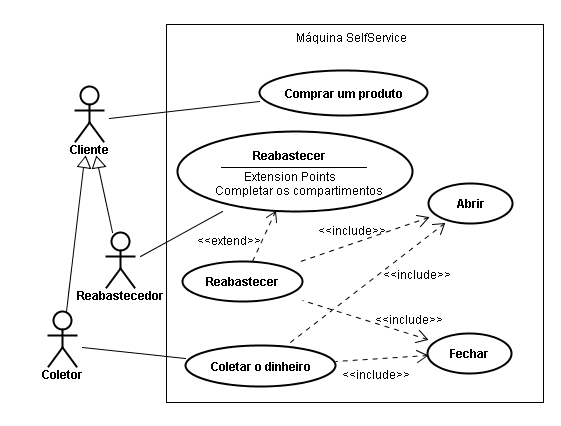
\includegraphics[scale=0.6]{imagens/DiagramaCasoDeUso.png} 
	\newline \textbf{Fonte}: (Própria, 2021).
	\label{fig:CasoDeUso}
\end{figure}

\begin{figure}[htb]
	\centering
	\caption{Exemplo de diagrama de atividade.}
	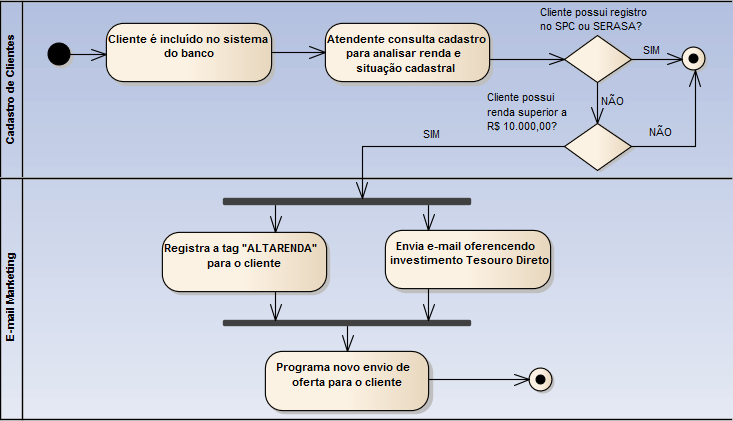
\includegraphics[scale=0.6]{imagens/DiagramaAtividades.png} 
	\newline \textbf{Fonte}: \cite{Ventura2018}.
	\label{fig:Atividades}
\end{figure}
